\documentclass[journal]{IEEEtran}
\usepackage{amsmath,amssymb}
\usepackage{booktabs}
\usepackage{multirow}
\usepackage{graphicx}
\usepackage{xcolor}
\usepackage{tikz}
\usetikzlibrary{positioning,arrows.meta,shapes.geometric,fit}
\usepackage{pgfplots}
\pgfplotsset{compat=1.16}
\usepackage[hidelinks]{hyperref}
\usepackage{cite}

\newcommand{\sfn}{SchemaFlexTabNet-QC}
\newcommand{\htn}{HybridTabNet-QC}

\begin{document}

\title{Duplicate Contamination, Schema Loss, and Cross-Cohort Generalization in Public Cardiovascular Risk Benchmarks: A Reproducibility Audit and a Schema-Flexible Tabular Transformer}

\author{\IEEEauthorblockN{Raja Rathan Paida}
\IEEEauthorblockA{Department of Artificial Intelligence\\
Sardar Vallabhbhai National Institute of Technology (SVNIT), Surat 395007, India\\
Email: paida.rajarthan@gmail.com}}

\maketitle

\begin{abstract}
Public cardiovascular-risk benchmarks are routinely used to report accuracies above 90\%, yet duplicated records, cross-cohort patient overlap, and schema loss during dataset merging receive little scrutiny. We audit six open data sources (74{,}013 non-overlapping patients after quality control) and show that (i)~723 of 1{,}025 rows (70.5\%) in a widely used Kaggle heart-disease copy are exact duplicates, so a random 80/20 split places 97.1\% of test rows in the training set and inflates accuracy to 98.5\%, versus 77.1\% after deduplication; (ii)~all 270 UCI Statlog records duplicate Cleveland records; (iii)~inner-join harmonization discards unshared features and drives zero-shot cross-cohort AUROC down to 0.535--0.713; and (iv)~duplicates are too few (1.02\%) to explain a published 90.1\% accuracy on a 71{,}025-row pool, where a 70/15/15 reproduction gives about 73\% with or without them. We propose \sfn{}, a feature-tokenizing transformer that models only the variables each cohort actually observes, trained with feature dropout, an auxiliary hypertension concept head and a monotonicity penalty, and deployed with temperature-scaled conformal abstention. Under leave-one-cohort-out (LOCO) evaluation it reaches a mean AUROC of 0.763, versus 0.611 for inner-join LightGBM and 0.740 for NaN-aware union-schema LightGBM; against the latter, no per-cohort difference is significant after Holm correction. At 50\% test-time missingness it keeps 0.712 AUROC versus 0.613 for native-NaN LightGBM. Conformal sets calibrated on source cohorts under-cover on held-out hospitals (84.2--88.7\% against a nominal 90\%). Outcome definitions differ across cohorts, and seed-to-seed variance is not yet quantified.
\end{abstract}

\begin{IEEEkeywords}
Cardiovascular risk prediction, tabular transformers, data leakage, multi-cohort harmonization, missing data, conformal prediction, reproducibility.
\end{IEEEkeywords}

%=====================================================================
\section{Introduction}
\IEEEPARstart{C}{ardiovascular} disease (CVD) causes roughly 17.9 million deaths per year worldwide. Machine-learning risk models are attractive for screening, but accuracies published on public benchmarks frequently exceed what noisy routine records can support, and they rarely survive transfer to a new hospital. Two well-documented sources of optimism are leakage between training and test data~\cite{kapoor2023} and near-duplicate records in benchmark files~\cite{barz2020}. A third, specific to multi-source clinical work, is the harmonization step itself: merging cohorts through an inner join keeps only the columns present everywhere and silently discards the most diagnostic variables of specialist cohorts (chest-pain type, exercise ECG response, vessel counts).

A recent study, \htn{}~\cite{mahmud2026}, reports 90.1\% accuracy and 93.6\% AUROC on a merger of two Kaggle datasets, using a transformer encoder fused with engineered meta-features (BMI, pulse pressure, and a cholesterol--glucose product). Motivated by the gap between that figure and what we observe on clean data, this paper makes four contributions:
\begin{enumerate}
\item \textbf{A data audit} of six public sources quantifying exact-duplicate contamination, cross-cohort patient overlap and physiologically implausible records, with a deterministic plausibility gatekeeper and a reproducible audit log.
\item \textbf{A reproducibility analysis} of~\cite{mahmud2026} that documents internal inconsistencies, bounds what the duplicate issue can explain, and reports a 70/15/15 reproduction of the published setup.
\item \textbf{\sfn{}}, a schema-flexible tokenizing transformer that trains across cohorts with non-identical columns, with physiological regularizers and conformal abstention.
\item \textbf{A leave-one-cohort-out benchmark} against strong baselines, including a NaN-aware union-schema gradient-boosting model, with Holm-corrected DeLong tests, ablations, missingness stress tests against native-NaN trees, a conformal cohort-shift audit, and subgroup, federated and decision-curve analyses.
\end{enumerate}
The paper is organized as follows. Section~\ref{sec:related} reviews related work, Section~\ref{sec:data} describes data and quality control, Section~\ref{sec:audit} presents the audit, Section~\ref{sec:method} the method, Section~\ref{sec:protocol} the protocol, Section~\ref{sec:results} the results, Section~\ref{sec:discussion} the discussion and limitations, and Section~\ref{sec:conclusion} concludes.

%=====================================================================
\section{Related Work}\label{sec:related}
\textbf{Tabular deep learning.} FT-Transformer~\cite{gorishniy2021}, TabNet~\cite{arik2021} and SAINT~\cite{somepalli2021} show that attention over feature tokens is competitive on tabular data, although gradient-boosted trees such as LightGBM~\cite{ke2017} remain strong baselines. Our tokenizer follows the feature-token idea but treats the \emph{set of observed features} as the input, so unobserved columns are masked rather than imputed.

\textbf{Domain knowledge in models.} Concept bottleneck models~\cite{koh2020} supervise intermediate, human-interpretable concepts, and monotonic models~\cite{gupta2016} encode the prior that risk should not fall as a harmful marker rises. We use both as soft regularizers rather than hard architectural constraints.

\textbf{Calibration and abstention.} Temperature scaling~\cite{guo2017} and conformal prediction~\cite{vovk2005,angelopoulos2023} provide calibrated probabilities and set-valued predictions with finite-sample coverage under exchangeability. That assumption fails under cohort shift~\cite{tibshirani2019,barber2023}, which matters for our setting and which we measure directly (Section~\ref{sec:conformal}).

\textbf{Reporting standards.} TRIPOD+AI~\cite{collins2024} and leakage checklists~\cite{kapoor2023} motivate the audit-first design of this work.

%=====================================================================
\section{Data and Quality Control}\label{sec:data}
\subsection{Sources}
We use six public sources: UCI Heart Disease from four institutions (Cleveland, Hungarian, Switzerland, VA Long Beach)~\cite{dua2019,detrano1989}; the Kaggle heart-disease copy (1{,}025 rows); the Sulianova cardiovascular dataset (70{,}000 examination records); a Framingham teaching subset (4{,}240 records)~\cite{dawber1951}; UCI Statlog Heart (270 records); and the Z-Alizadeh Sani angiography cohort (303 records; 56 clinical and laboratory variables)~\cite{alizadehsani2013}.

\subsection{Canonical schema}
A registry defines 22 union features: continuous variables (age, systolic and diastolic blood pressure, BMI, pulse pressure, cholesterol, maximum heart rate, ST depression), categorical variables (sex, ATP-III cholesterol tier, glucose tier, chest-pain type, exercise angina, smoking), and one auxiliary concept, Stage~2 hypertension (SBP $\ge$ 140 or DBP $\ge$ 90~mmHg). Variables that a cohort does not record are left \emph{absent}, not zero-filled.

\subsection{Plausibility gatekeeper}
Instead of a statistical $|Z|>3$ filter, records are rejected if they violate physiological bounds (age 18--110~y; SBP 60--260; DBP 40--160~mmHg; BMI 12--70; cholesterol 80--650~mg/dL; heart rate 50--230~bpm; ST depression 0--10~mm) or hemodynamic consistency (SBP $-$ DBP $\ge$ 10~mmHg). Exact patient-level duplicates are removed. Table~\ref{tab:audit} gives the audit log. The eight clean cohorts sum to 74{,}283 records; excluding the 270 Statlog rows that duplicate Cleveland leaves 74{,}013 non-overlapping patients, which is the pool used throughout the paper. Sulianova contributes 92.6\% of these (68{,}568 of 74{,}013), a fact that shapes several conclusions below.

\begin{table*}[t]
\caption{Cohort summary. ``Cardiology variables'' denotes chest-pain type, peak heart rate, exercise angina, ST depression and vessel count. Outcome definitions differ across sources and are mapped to one binary label.}
\label{tab:cohorts}
\centering\footnotesize
\begin{tabular}{p{3.2cm}rp{4.6cm}p{2.9cm}p{3.6cm}}
\toprule
Source & Clean $N$ & Outcome construct & Cardiology variables & Role in this study\\
\midrule
Sulianova CVD & 68{,}568 & Presence of CVD at examination & Not recorded & Training (all LOCO folds)\\
Framingham subset & 4{,}238 & Incident CHD during follow-up & Not recorded & Training; held-out unit\\
UCI Cleveland & 303 & Angiographic coronary disease & Recorded & Training; held-out unit\\
UCI Hungarian & 293 & Angiographic coronary disease & Recorded (partly missing) & Training; held-out unit\\
UCI VA + Switzerland & 308 & Angiographic coronary disease & Recorded (partly missing) & Training; held-out unit\\
Z-Alizadeh Sani & 303 & Coronary stenosis on angiography & Recorded (plus lab panel) & Training; held-out unit\\
UCI Statlog & 270 & Angiographic coronary disease & Recorded & Excluded (duplicates Cleveland)\\
Kaggle heart copy & 302 unique & Angiographic coronary disease & Recorded & Audit only\\
\bottomrule
\end{tabular}
\end{table*}

\begin{table}[t]
\caption{Quality-control audit log.}
\label{tab:audit}
\centering\footnotesize
\begin{tabular}{lrrrr}
\toprule
Source & Raw & Dup. & Implaus. & Clean\\
\midrule
UCI Cleveland & 303 & 0 & 0 & 303\\
UCI Hungarian & 294 & 1 & 0 & 293\\
UCI Switzerland & 123 & 0 & 11 & 112\\
UCI VA Long Beach & 200 & 3 & 1 & 196\\
Sulianova CVD & 70{,}000 & 58 & 1{,}374 & 68{,}568\\
Framingham subset & 4{,}240 & 0 & 2 & 4{,}238\\
UCI Statlog & 270 & 0 & 0 & 270\\
Z-Alizadeh Sani & 303 & 0 & 0 & 303\\
\midrule
\emph{Kaggle heart copy} & \emph{1{,}025} & \emph{723} & \emph{0} & \emph{302}\\
\bottomrule
\end{tabular}
\end{table}

%=====================================================================
\section{Reproducibility Audit}\label{sec:audit}
\subsection{Duplicate leakage and cohort overlap}
The Kaggle heart copy contains only 302 unique patients; the remaining 723 rows (70.5\%) are exact copies. Under a random 80/20 split, 199 of 205 test rows (97.1\%) have an identical twin in the training set. Evaluating on that split yields near-perfect scores that vanish once duplicates are removed (Table~\ref{tab:leak}). A signature match on age, sex, resting blood pressure, cholesterol, peak heart rate and ST depression further shows that all 270 Statlog patients are identical to Cleveland patients, so training on one and testing on the other is leakage; we excluded the overlap from every cross-cohort experiment.

\begin{table}[t]
\caption{Effect of duplicate leakage on a small cardiology benchmark.}
\label{tab:leak}
\centering\footnotesize
\begin{tabular}{p{2.6cm}p{2.3cm}rr}
\toprule
Setup & Data & Acc. & AUROC\\
\midrule
Random split, duplicates kept & Kaggle copy (1{,}025) & 98.54\% & 0.9980\\
Deduplicated patient split & Cleveland (302) & 77.05\% & 0.8593\\
Examination data only & Sulianova (68{,}568) & 73.21\% & 0.7943\\
\bottomrule
\end{tabular}
\end{table}

\subsection{Observations on the published \htn{} results}
We did not have access to code or splits for~\cite{mahmud2026}, and we do not claim to know why its figures differ from ours. We report only what can be checked from the article itself, plus a reproduction of its stated split.
\begin{itemize}
\item \textbf{Inconsistent confusion matrices.} The text describes a matrix with 980/1{,}100 negatives and 990/1{,}100 positives correct (accuracy 89.5\%), whereas Fig.~2 of that article shows 4{,}795/533/395/4{,}930 on 10{,}653 samples, implying accuracy 91.3\% and positive-class recall 0.926, against 0.90 in its Table~1.\footnote{The project implementation reports list an alternative matrix (5{,}044/4{,}688/444/477). We use the values from the published LaTeX, which are consistent with the ``balanced 5{,}328 vs.\ 5{,}325'' description. Readers should verify against the published figure.}
\item \textbf{Class balance.} The test set is described as balanced (5{,}328 vs.\ 5{,}325), while the preprocessing section describes a roughly 1:2 minority-to-majority imbalance with class weights 0.45/0.55.
\item \textbf{Test-set size.} 10{,}653 equals 15\% of 71{,}025, the sum of the raw rows of the two Kaggle files ($1{,}025+70{,}000$). This is consistent with the duplicated 1{,}025-row copy having been used, and with little row removal despite the described outlier filtering.
\item \textbf{Limits of the duplicate explanation.} The 723 duplicate rows are $723/71{,}025=1.02\%$ of the pooled set. Even if every duplicate were classified correctly, raising their accuracy from about 73\% to 100\% would lift overall accuracy by only about $0.0102\times(1-0.73)\approx 0.3$ percentage points. Duplicates therefore cannot by themselves explain 90.1\% accuracy on a pool that is 98.6\% Sulianova, where well-tuned models in our benchmark reach roughly 73--76\%.
\item \textbf{Engineered features are not architecture-specific.} Adding BMI, pulse pressure and tier features changes AUROC by $+0.0014$ (MLP) to $+0.0124$ (logistic regression) across seven model families (Section~\ref{sec:pooled}). Work~\cite{mahmud2026} states that baselines were retrained under the same pipeline, so we do not allege unequal treatment; we show only that the features help every model.
\end{itemize}

\subsection{Reproduction of the 70/15/15 setup}
We applied the stated 70/15/15 train/validation/test protocol to (a)~the raw 71{,}025-row pool, (b)~the same pool with the 723 Kaggle duplicates removed, and (c)~Sulianova alone, using the same hemodynamic filtering in each case and a LightGBM classifier with default hyperparameters and the engineered meta-features described in~\cite{mahmud2026}. Table~\ref{tab:repro} shows that all three configurations land at about 73\% accuracy and 0.795--0.799 AUROC. Keeping the duplicates changes accuracy by $+0.30$ points, in line with the bound above. We could not reproduce 90.1\% with these features and this protocol. The discrepancy may reflect preprocessing or reporting details that are not documented in the article; we cannot tell which, and we recommend release of splits and code.

\begin{table}[t]
\caption{Reproduction of the published 70/15/15 setup. Hemodynamic filtering reduces the row counts.}
\label{tab:repro}
\centering\footnotesize
\begin{tabular}{p{3.0cm}rrrr}
\toprule
Configuration & Clean $N$ & Test $N$ & Acc. (\%) & AUROC\\
\midrule
Pool, duplicates kept (71{,}025 raw) & 69{,}692 & 10{,}454 & 73.48 & 0.7978\\
Pool, deduplicated (70{,}302 raw) & 68{,}969 & 10{,}346 & 73.18 & 0.7954\\
Sulianova alone (70{,}000 raw) & 68{,}667 & 10{,}301 & 73.42 & 0.7987\\
\bottomrule
\end{tabular}
\end{table}

%=====================================================================
\section{Method: \sfn{}}\label{sec:method}
Fig.~\ref{fig:arch} summarizes the architecture.

\begin{figure}[t]
\centering
\resizebox{\columnwidth}{!}{%
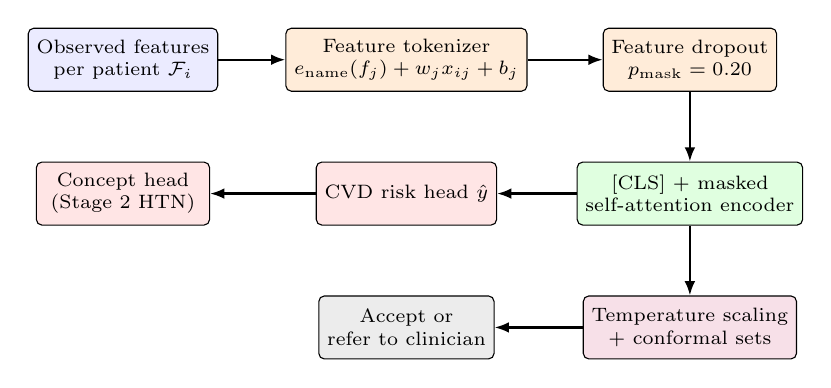
\begin{tikzpicture}[
  box/.style={draw,rounded corners=2pt,align=center,font=\scriptsize,minimum height=8mm,minimum width=22mm,inner sep=3pt},
  arr/.style={-{Latex[length=1.8mm]},thick}]
\node[box,fill=blue!8] (in) at (0,0) {Observed features\\per patient $\mathcal{F}_i$};
\node[box,fill=orange!15] (tok) at (3.6,0) {Feature tokenizer\\$e_{\mathrm{name}}(f_j)+w_jx_{ij}+b_j$};
\node[box,fill=orange!15] (drop) at (7.2,0) {Feature dropout\\$p_{\mathrm{mask}}=0.20$};
\node[box,fill=green!12] (enc) at (7.2,-1.7) {[CLS] + masked\\self-attention encoder};
\node[box,fill=red!10] (risk) at (3.6,-1.7) {CVD risk head $\hat y$};
\node[box,fill=red!10] (con) at (0,-1.7) {Concept head\\(Stage 2 HTN)};
\node[box,fill=purple!12] (cal) at (7.2,-3.4) {Temperature scaling\\+ conformal sets};
\node[box,fill=gray!15] (out) at (3.6,-3.4) {Accept or\\refer to clinician};
\draw[arr] (in)--(tok); \draw[arr] (tok)--(drop); \draw[arr] (drop)--(enc);
\draw[arr] (enc)--(risk); \draw[arr] (risk)--(con); \draw[arr] (enc)--(cal);
\draw[arr] (cal)--(out);
\end{tikzpicture}}
\caption{\sfn{} pipeline. Only observed features are tokenized; absent features are masked in attention. A monotonicity penalty acts on $\partial\hat y/\partial x_k$ during training.}
\label{fig:arch}
\end{figure}

\subsection{Schema-flexible tokenizer}
For patient $i$ with observed feature set $\mathcal{F}_i$, each observed feature $j\in\mathcal{F}_i$ becomes a token
\begin{equation}
z_{ij}=e_{\mathrm{name}}(f_j)+w_j\,x_{ij}+b_j,
\end{equation}
where $e_{\mathrm{name}}(f_j)\in\mathbb{R}^d$ is a learned feature-identity embedding and $(w_j,b_j)$ is a feature-specific linear projection (categorical variables use learned value embeddings). Continuous inputs are z-scored with training statistics. A learnable \texttt{[CLS]} token is prepended and a key-padding mask removes unobserved features from attention, so no inner join, zero-fill or imputation is needed. The encoder has 2 layers, 4 heads, width $d=64$, feed-forward width 128 and dropout 0.10.

\subsection{Feature dropout}
During training each observed token is dropped with probability $p_{\mathrm{mask}}=0.20$, simulating hospitals that supply only part of the panel and forcing the encoder not to rely on any single variable.

\subsection{Concept head and monotonicity}
The \texttt{[CLS]} representation also predicts Stage~2 hypertension, giving $\mathcal{L}_{\mathrm{concept}}$ (binary cross-entropy). Monotonicity is encouraged in two ways for the set of harmful markers $\mathcal{M}=\{$age, SBP, cholesterol, ST depression$\}$. First, the logit contains a residual branch with softplus-constrained, hence non-negative, weights:
\begin{equation}
\hat z_i=\mathbf{w}_{\mathrm{out}}^{\top}\mathbf{h}^{\mathrm{CLS}}_i+b_0+\sum_{k\in\mathcal{M}}\mathrm{softplus}(w_k)\,x_{ik}\,\mathbb{I}[x_{ik}\ \text{observed}],
\end{equation}
with $\hat y_i=\sigma(\hat z_i)$. Second, an input-gradient penalty computed by automatic differentiation,
\begin{equation}
\mathcal{L}_{\mathrm{mono}}=\frac{1}{|\mathcal{M}|}\sum_{k\in\mathcal{M}}\mathrm{ReLU}\!\left(-\frac{\partial \hat y_i}{\partial x_{i,k}}\right)\mathbb{I}[x_{i,k}\ \text{observed}].
\end{equation}
The total loss is
\begin{equation}
\mathcal{L}=\mathcal{L}_{\mathrm{BCE}}+\lambda_1\mathcal{L}_{\mathrm{concept}}+\lambda_2\mathcal{L}_{\mathrm{mono}},
\end{equation}
with $\lambda_1=0.10$ and $\lambda_2=1.20$. Because the attention path is unconstrained, neither mechanism guarantees monotonicity; we therefore \emph{measure} violations (Section~\ref{sec:ablation}).

\subsection{Calibration and abstention}
Temperature scaling is fitted by L-BFGS on held-out validation data. Split conformal prediction at $\alpha=0.10$ then yields a label set $\mathcal{C}(x)\subseteq\{0,1\}$. If $|\mathcal{C}(x)|=1$ the prediction is accepted; otherwise the case is flagged for clinician review. A Mondrian variant computes non-conformity quantiles separately per sex.

\subsection{Conformal procedure}
Let $p(x)$ be the temperature-scaled probability of disease and define the non-conformity score $s(x,y)=1-p_y(x)$. On a calibration set of $n$ labeled patients, let $\hat q$ be the $\lceil (n+1)(1-\alpha)\rceil/n$ empirical quantile of the scores $s(x_i,y_i)$. The prediction set is
\begin{equation}
\mathcal{C}(x)=\{y\in\{0,1\}:\ s(x,y)\le \hat q\}.
\end{equation}
Under exchangeability of calibration and test data, $\Pr[Y\in\mathcal{C}(X)]\ge 1-\alpha$. The Mondrian variant computes $\hat q_g$ separately for each sex $g$, which targets the group-conditional guarantee $\Pr[Y\in\mathcal{C}(X)\mid G=g]\ge 1-\alpha$, again under within-group exchangeability. A case is \emph{accepted} when $|\mathcal{C}(x)|=1$, and \emph{referred} when $\mathcal{C}(x)=\{0,1\}$ or $\emptyset$.

We keep two quantities strictly apart. \emph{Set coverage} is $\Pr[Y\in\mathcal{C}(X)]$, the quantity the conformal guarantee is about. The \emph{acceptance rate} is the fraction of patients with $|\mathcal{C}(x)|=1$; it is a selective-prediction rate and carries no coverage guarantee. In leave-one-cohort-out use, calibration scores come from source cohorts while test patients come from a different hospital, so $P_{\mathrm{source}}(X,Y)\neq P_{\mathrm{target}}(X,Y)$ and exchangeability does not hold; we measure the resulting coverage loss in Section~\ref{sec:conformal}.

\subsection{Schema-aware federated averaging}
In the federated simulation each hospital node $h$ observes a feature subset $\mathcal{F}_h$. Parameters shared across features (transformer blocks, \texttt{[CLS]}, heads) are averaged over all nodes, weighted by local sample size $n_h$:
\begin{equation}
\theta_{\mathrm{shared}}\leftarrow\sum_h \frac{n_h}{\sum_{h'}n_{h'}}\,\theta^{(h)}_{\mathrm{shared}}.
\end{equation}
Feature-specific parameters $\theta_j=(e_{\mathrm{name}}(f_j),w_j,b_j)$ are averaged only over the nodes $H_j=\{h: j\in\mathcal{F}_h\}$ that observe feature $j$:
\begin{equation}
\theta_j\leftarrow\sum_{h\in H_j}\frac{n_h}{\sum_{h'\in H_j}n_{h'}}\,\theta^{(h)}_j.
\end{equation}
This prevents embeddings of a feature from being diluted by nodes that never see it.

\subsection{Evaluation metrics}
Calibration is summarized by the expected calibration error over $B$ equal-width probability bins,
\begin{equation}
\mathrm{ECE}=\sum_{b=1}^{B}\frac{|S_b|}{N}\,\bigl|\mathrm{acc}(S_b)-\mathrm{conf}(S_b)\bigr|,
\end{equation}
and by the Brier score $\frac{1}{N}\sum_i(\hat y_i-y_i)^2$. Clinical utility at decision threshold $p_t$ is the net benefit
\begin{equation}
\mathrm{NB}(p_t)=\frac{TP}{N}-\frac{FP}{N}\cdot\frac{p_t}{1-p_t},
\end{equation}
compared with the treat-all strategy $\mathrm{NB}_{\mathrm{all}}=\pi-(1-\pi)\,p_t/(1-p_t)$, where $\pi$ is prevalence~\cite{vickers2006}.

%=====================================================================
\section{Experimental Protocol}\label{sec:protocol}
\textbf{Evaluation partitions.} Each experiment uses one stated partition. (i)~The pooled benchmark is stratified five-fold cross-validation on the 74{,}013 non-overlapping patients. (ii)~The LOCO and DeLong analyses hold out each of five units in turn: UCI Hungarian ($N{=}293$), UCI VA+Switzerland (308), UCI Cleveland deduplicated (303), Z-Alizadeh Sani (303) and Framingham (4{,}238); the model trains on the remaining non-overlapping cohorts, and Statlog is excluded throughout. (iii)~The missingness stress test and the ablation use a held-out 15\% stratified multi-cohort test partition, so their values are not comparable with the LOCO table. (iv)~Subgroup, decision-curve and bootstrap analyses use the 270-patient Statlog/Cleveland-overlap evaluation (model trained without Cleveland); these patients are a subset of Cleveland, so these results are not independent of the Cleveland LOCO row.

\textbf{Baselines.} (a)~Inner-join LightGBM on shared features; (b)~union-schema LightGBM with native missing-value handling; (c)~\htn{} \emph{re-implemented from the published description} with an inner-join merge, since no official code is available. For missingness stress tests we add native-NaN LightGBM and XGBoost and median-imputed LightGBM. A pooled five-fold benchmark covers seven classical and neural models with and without engineered meta-features.

\textbf{Metrics and tests.} AUROC, accuracy, Brier score and expected calibration error (ECE). Paired AUROC differences use DeLong's test~\cite{delong1988} with Holm--Bonferroni correction across the five held-out cohorts; clinical utility is assessed with decision-curve analysis~\cite{vickers2006}; federated experiments follow FedAvg~\cite{mcmahan2017}.

\textbf{Remaining statistical work.} Table values are single runs. Bootstrap intervals (1{,}000 patient resamples) are reported only for the 270-patient analysis, and mean $\pm$ standard deviation over at least five seeds for the neural models remains outstanding.

\textbf{Implementation.} The encoder configuration is given in Section~\ref{sec:method}. Training uses AdamW with learning rate $1.5\times10^{-3}$, weight decay $10^{-4}$, batch size 256, and 16 epochs. Results are from a single seed; multi-seed variance is not yet reported. Code and configuration are in the repository listed under Data and Code Availability.

%=====================================================================
\section{Results}\label{sec:results}
\subsection{Pooled benchmark}\label{sec:pooled}
On pooled stratified five-fold cross-validation (74{,}013 patients), LightGBM with raw plus engineered features reaches AUROC 0.8249 and accuracy 75.98\% (75.39\% with raw features only). XGBoost, random forest and CatBoost lie within 0.004 AUROC, MLP and TabNet reach about 0.811, and logistic regression 0.768 (Table~\ref{tab:pooled}). Among the models tested these values form an empirical ceiling for this pool, and they are far below 90\%. Engineered features help every model by between $+0.0014$ and $+0.0124$ AUROC.

\begin{table}[t]
\caption{Pooled 5-fold benchmark: AUROC with raw features (A) and with engineered meta-features (B); accuracy for B.}
\label{tab:pooled}
\centering\footnotesize
\begin{tabular}{lcccc}
\toprule
Model & A & B & $\Delta$ & Acc.\ B (\%)\\
\midrule
Logistic regression & 0.7554 & 0.7678 & $+0.0124$ & 70.19\\
Random forest & 0.8195 & 0.8244 & $+0.0049$ & 75.85\\
XGBoost & 0.8186 & 0.8247 & $+0.0061$ & 75.95\\
LightGBM & 0.8187 & 0.8249 & $+0.0062$ & 75.98\\
CatBoost & 0.8152 & 0.8215 & $+0.0063$ & 75.60\\
MLP & 0.8096 & 0.8110 & $+0.0014$ & 74.86\\
TabNet & 0.8078 & 0.8105 & $+0.0027$ & 74.87\\
\bottomrule
\end{tabular}
\end{table}

\subsection{Zero-shot cross-cohort transfer}
Table~\ref{tab:loco} and Fig.~\ref{fig:loco} show LOCO transfer. Inner-join models are weak (mean AUROC 0.611 for LightGBM and 0.645 for the re-implemented \htn{}) because the shared columns exclude chest-pain type, exercise ECG variables and vessel counts. Retaining the union schema is the decisive change: NaN-aware LightGBM already reaches 0.740. \sfn{} reaches 0.763, a mean gain of $+0.023$ over that stronger baseline, driven by Z-Alizadeh ($+0.102$) and Hungarian ($+0.022$); it is lower on VA+Switzerland ($-0.004$) and Cleveland ($-0.013$).

Table~\ref{tab:delong} gives paired DeLong tests. Against the re-implemented inner-join \htn{}, \sfn{} is significantly better on Hungarian ($p<10^{-10}$), VA+Switzerland ($p{=}5.6\times10^{-4}$) and Cleveland ($p{=}2.1\times10^{-6}$), and not significantly different on Z-Alizadeh ($p{=}0.84$) or Framingham ($p{=}0.71$). Against the union-schema LightGBM, the most informative comparison, the Z-Alizadeh gain is nominally significant (raw $p{=}0.037$) but no cohort survives Holm correction (adjusted $p\ge 0.18$). We therefore treat \sfn{} as statistically comparable to union-schema LightGBM on these cohorts, not superior to it.

\begin{table*}[t]
\caption{Zero-shot LOCO AUROC. Hybrid = re-implemented \htn{} with inner join; Union LGBM = NaN-aware LightGBM on the union schema. The mean row is the unweighted mean of the five per-cohort values. Bold marks the best value per row.}
\label{tab:loco}
\centering\footnotesize
\begin{tabular}{lccccc}
\toprule
Held-out cohort ($N$) & Inner-join LGBM & Hybrid (re-impl.) & Union LGBM & \sfn{} & $\Delta$ vs.\ union\\
\midrule
Hungarian (293) & 0.5917 & 0.6111 & 0.8423 & \textbf{0.8641} & $+0.0218$\\
VA+Switzerland (308) & 0.5353 & 0.5451 & \textbf{0.7280} & 0.7241 & $-0.0039$\\
Cleveland dedup.\ (303) & 0.5705 & 0.6785 & \textbf{0.8566} & 0.8433 & $-0.0133$\\
Z-Alizadeh Sani (303) & 0.6881 & \textbf{0.7126} & 0.6028 & 0.7043 & $+0.1015$\\
Framingham (4{,}238) & 0.6701 & 0.6750 & 0.6695 & \textbf{0.6778} & $+0.0083$\\
\midrule
Unweighted mean & 0.6111 & 0.6445 & 0.7398 & 0.7627 & $+0.0229$\\
\bottomrule
\end{tabular}
\end{table*}

\begin{table*}[t]
\caption{Paired DeLong tests for \sfn{}. ``Union'' = union-schema NaN-aware LightGBM, with Holm--Bonferroni adjustment across the five cohorts. ``Hybrid'' = re-implemented inner-join \htn{} (unadjusted $p$). n.s.\ = not significant at 0.05.}
\label{tab:delong}
\centering\footnotesize
\begin{tabular}{lrcccccc}
\toprule
Held-out cohort & $N$ & $\Delta$ vs.\ union & DeLong $z$ & Raw $p$ & Holm $p$ & Sig.\ (Holm) & $p$ vs.\ Hybrid\\
\midrule
Hungarian & 293 & $+0.0218$ & 1.413 & 0.158 & 0.631 & n.s. & $<10^{-10}$\\
VA+Switzerland & 308 & $-0.0039$ & $-0.255$ & 0.798 & 1.000 & n.s. & $5.6\times10^{-4}$\\
Cleveland dedup. & 303 & $-0.0133$ & $-0.760$ & 0.447 & 1.000 & n.s. & $2.1\times10^{-6}$\\
Z-Alizadeh Sani & 303 & $+0.1015$ & 2.087 & 0.037 & 0.185 & n.s. & 0.84 (n.s.)\\
Framingham & 4{,}238 & $+0.0083$ & 0.722 & 0.470 & 1.000 & n.s. & 0.71 (n.s.)\\
\bottomrule
\end{tabular}
\end{table*}

\begin{figure}[t]
\centering
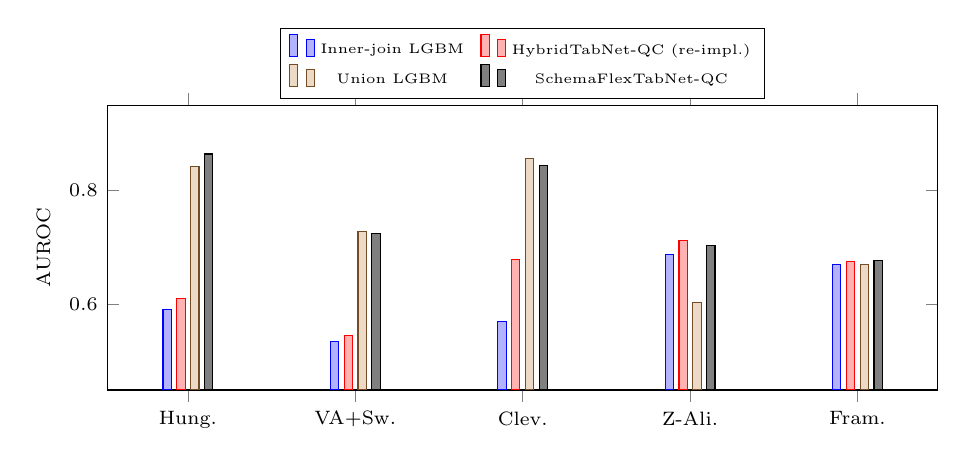
\begin{tikzpicture}
\begin{axis}[ybar,width=\columnwidth,height=5.2cm,bar width=3pt,
  symbolic x coords={Hung.,VA+Sw.,Clev.,Z-Ali.,Fram.},xtick=data,
  x tick label style={font=\scriptsize},y tick label style={font=\scriptsize},
  ylabel={AUROC},ylabel style={font=\scriptsize},ymin=0.45,ymax=0.95,
  legend style={font=\tiny,at={(0.5,1.02)},anchor=south,legend columns=2,/tikz/every even column/.append style={column sep=4pt}},
  enlarge x limits=0.12]
\addplot coordinates {(Hung.,0.5917) (VA+Sw.,0.5353) (Clev.,0.5705) (Z-Ali.,0.6881) (Fram.,0.6701)};
\addplot coordinates {(Hung.,0.6111) (VA+Sw.,0.5451) (Clev.,0.6785) (Z-Ali.,0.7126) (Fram.,0.6750)};
\addplot coordinates {(Hung.,0.8423) (VA+Sw.,0.7280) (Clev.,0.8566) (Z-Ali.,0.6028) (Fram.,0.6695)};
\addplot coordinates {(Hung.,0.8641) (VA+Sw.,0.7241) (Clev.,0.8433) (Z-Ali.,0.7043) (Fram.,0.6778)};
\legend{Inner-join LGBM,\htn{} (re-impl.),Union LGBM,\sfn{}}
\end{axis}
\end{tikzpicture}
\caption{Zero-shot AUROC by held-out cohort (data of Table~\ref{tab:loco}).}
\label{fig:loco}
\end{figure}

\subsection{Ablation and monotonicity}\label{sec:ablation}
Table~\ref{tab:abl} isolates each component on the held-out 15\% multi-cohort partition. The tokenizer produces by far the largest effect ($+0.222$ AUROC from variant 1 to 2). Feature dropout adds $+0.004$ AUROC and lowers monotonicity violations from 19.2\% to 4.2\%. The concept head changes AUROC by only $+0.0007$ and raises violations to 13.0\%, so we do not claim a discrimination benefit from it; any value it has is interpretive rather than predictive. Adding the monotone skip path, the gradient penalty ($\lambda_2=1.20$) and temperature scaling gives the best accuracy (80.20\%), ECE (0.057) and a violation rate of 0.26\% on synthetic $+0.5$~SD perturbations of SBP and cholesterol. These are single-run figures without confidence intervals, and the evaluation split differs from that of Table~\ref{tab:loco}.

\begin{table}[t]
\caption{Component ablation on the held-out 15\% multi-cohort partition. Viol.\ = counterfactual monotonicity violations (\%).}
\label{tab:abl}
\centering\footnotesize
\begin{tabular}{p{2.9cm}rrrr}
\toprule
Variant & AUROC & Acc. & ECE & Viol.\\
\midrule
1. Inner-join, shared feats. & 0.6342 & 59.73 & 0.1368 & 15.04\\
2. + Schema tokenizer & 0.8560 & 75.77 & 0.1672 & 19.23\\
3. + Feature dropout & 0.8604 & 77.13 & 0.1008 & 4.18\\
4. + Concept head & 0.8611 & 77.82 & 0.1081 & 12.97\\
5. + Mono.\ + temperature & 0.8652 & 80.20 & 0.0572 & 0.26\\
\bottomrule
\end{tabular}
\end{table}

\subsection{Conformal abstention and cohort shift}\label{sec:conformal}
At $\alpha=0.10$ the model accepts 36.6--78.9\% of patients depending on the cohort (Table~\ref{tab:conf}). On accepted cases AUROC rises by 0.03--0.09 and accuracy by 5--10 points on four cohorts; on Framingham accuracy does not improve (51.3\% to 51.2\%). The accepted fraction is a \emph{selective-prediction rate}, not conformal coverage.

Set coverage tells a different story. With calibration scores taken from source cohorts, empirical coverage $\Pr[Y\in\mathcal{C}(X)]$ on the held-out hospital falls to 84.2--88.7\%, below the nominal 90\%, confirming that exchangeability is violated. Re-calibrating on a labeled slice of the target cohort restores coverage to 90.0--90.4\%. This repair needs labeled target data, so it is not available in a true zero-shot deployment. On the Statlog/Cleveland-overlap analysis, the only one with bootstrap intervals, AUROC is 0.882 (95\% CI 0.839--0.918) at full coverage; this is a 270-patient subset of Cleveland trained without Cleveland and is not independent of the 0.843 Cleveland LOCO figure.

\begin{table*}[t]
\caption{Conformal abstention at $\alpha=0.10$ under cohort shift. Accepted = fraction with a singleton set. Coverage = $\Pr[Y\in\mathcal{C}(X)]$ with nominal value 90\%, using source-cohort calibration (Src.) or a labeled slice of the target cohort (Tgt.). AUROC and accuracy: all patients $\rightarrow$ accepted patients.}
\label{tab:conf}
\centering\footnotesize
\begin{tabular}{lrcccc}
\toprule
Held-out cohort & Accepted & Src.\ coverage & Tgt.\ coverage & AUROC & Accuracy (\%)\\
\midrule
Hungarian & 78.2\% & 88.7\% & 90.4\% & .864 $\rightarrow$ .893 & 76.8 $\rightarrow$ 85.2\\
VA+Switzerland & 72.7\% & 86.4\% & 90.3\% & .724 $\rightarrow$ .771 & 74.0 $\rightarrow$ 83.5\\
Cleveland dedup. & 78.9\% & 88.1\% & 90.1\% & .843 $\rightarrow$ .876 & 73.6 $\rightarrow$ 78.7\\
Z-Alizadeh Sani & 36.6\% & 84.2\% & 90.1\% & .704 $\rightarrow$ .790 & 62.7 $\rightarrow$ 72.1\\
Framingham & 64.1\% & 87.3\% & 90.0\% & .678 $\rightarrow$ .706 & 51.3 $\rightarrow$ 51.2\\
\bottomrule
\end{tabular}
\end{table*}

\subsection{Robustness to missing data}
Table~\ref{tab:miss} and Fig.~\ref{fig:miss} show AUROC as 0--50\% of features are masked at test time, on the held-out 15\% partition. \sfn{} degrades from 0.852 to 0.712 and an unregularized tabular transformer from 0.838 to 0.699. The tree baselines now use native missing-value handling: at 50\% missingness \sfn{} exceeds native-NaN LightGBM by $+0.099$ AUROC, native-NaN XGBoost by $+0.078$ and median-imputed LightGBM by $+0.079$. These margins are smaller than those against median-imputed trees reported in earlier drafts, where the gap reached 0.15. Two cautions apply. At 0\% missingness the tree baselines (about 0.73) sit well below the pooled cross-validated LightGBM of Table~\ref{tab:pooled} (0.825); this gap likely reflects different partitions and tuning, and the absolute difference should be interpreted with care rather than taken as an apples-to-apples comparison. The 0.014--0.032 margin over the unregularized transformer is attributed to feature dropout but has not been separated from other differences.

\begin{table}[t]
\caption{AUROC under test-time missing features. Native = native missing-value handling; Med.\ = median imputation; Unreg.\ = unregularized transformer.}
\label{tab:miss}
\centering\footnotesize
\setlength{\tabcolsep}{3pt}
\begin{tabular}{rccccc}
\toprule
Missing & \sfn{} & Unreg. & Native LGBM & Native XGB & Med.\ LGBM\\
\midrule
0\%  & 0.8520 & 0.8377 & 0.7297 & 0.7265 & 0.7274\\
10\% & 0.8300 & 0.8018 & 0.7035 & 0.7051 & 0.7090\\
20\% & 0.8036 & 0.7767 & 0.6854 & 0.6940 & 0.6944\\
30\% & 0.7510 & 0.7294 & 0.6718 & 0.6822 & 0.6779\\
40\% & 0.7159 & 0.6955 & 0.6412 & 0.6575 & 0.6539\\
50\% & 0.7123 & 0.6985 & 0.6131 & 0.6341 & 0.6337\\
\bottomrule
\end{tabular}
\end{table}

\begin{figure}[t]
\centering
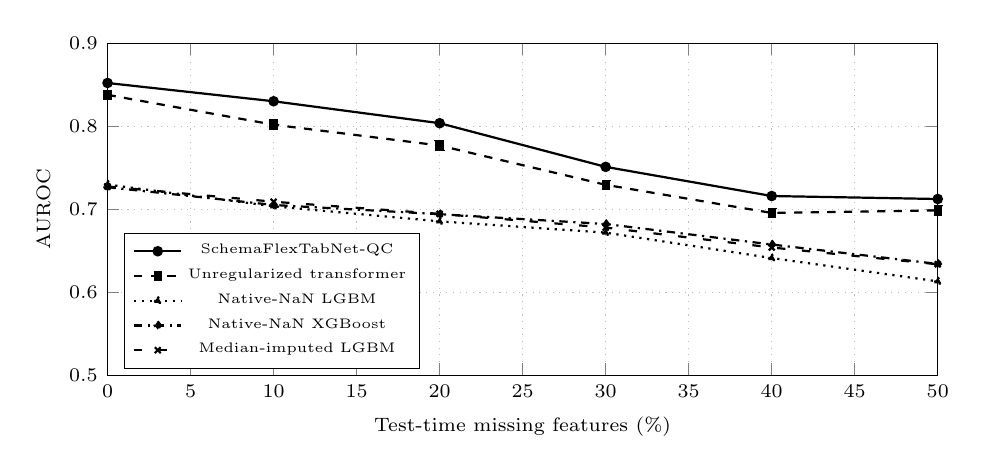
\begin{tikzpicture}
\begin{axis}[width=\columnwidth,height=5.8cm,xlabel={Test-time missing features (\%)},ylabel={AUROC},
  xlabel style={font=\scriptsize},ylabel style={font=\scriptsize},
  tick label style={font=\scriptsize},legend style={font=\tiny,at={(0.02,0.02)},anchor=south west},
  xmin=0,xmax=50,ymin=0.5,ymax=0.9,grid=major,grid style={dotted}]
\addplot[thick,mark=*,mark size=1.5pt] coordinates {(0,0.8520)(10,0.8300)(20,0.8036)(30,0.7510)(40,0.7159)(50,0.7123)};
\addplot[thick,dashed,mark=square*,mark size=1.5pt] coordinates {(0,0.8377)(10,0.8018)(20,0.7767)(30,0.7294)(40,0.6955)(50,0.6985)};
\addplot[thick,dotted,mark=triangle*,mark size=1.5pt] coordinates {(0,0.7297)(10,0.7035)(20,0.6854)(30,0.6718)(40,0.6412)(50,0.6131)};
\addplot[thick,dashdotted,mark=diamond*,mark size=1.5pt] coordinates {(0,0.7265)(10,0.7051)(20,0.6940)(30,0.6822)(40,0.6575)(50,0.6341)};
\addplot[thick,loosely dashed,mark=x,mark size=1.5pt] coordinates {(0,0.7274)(10,0.7090)(20,0.6944)(30,0.6779)(40,0.6539)(50,0.6337)};
\legend{\sfn{},Unregularized transformer,Native-NaN LGBM,Native-NaN XGBoost,Median-imputed LGBM}
\end{axis}
\end{tikzpicture}
\caption{Structured-missingness stress test (data of Table~\ref{tab:miss}).}
\label{fig:miss}
\end{figure}

\subsection{Fairness, federation and clinical utility}
\textbf{Subgroups.} On the 270-patient overlap cohort, male and female false-positive rates are 0.398 and 0.119 and sensitivities 0.86 and 0.80; the age $>65$ group has only 30 patients. In a separate 298-patient evaluation, marginal conformal calibration gave FPRs of 0.038 (male) and 0.186 (female); Mondrian calibration moved them to 0.173 and 0.246. It therefore \emph{halved} the inter-sex FPR gap, from 0.149 to 0.072 (a 51\% reduction), and lowered male FNR from 0.395 to 0.250, but it did not eliminate the gap and it raised the FPR of both groups. Subgroup samples are too small for confidence intervals to support firm conclusions.

\textbf{Federated simulation.} In a four-node simulation, schema-aware averaging (feature-specific parameters averaged only across nodes that observe the feature) reaches 0.767 AUROC after 10 rounds, versus 0.746 for isolated models and 0.875 for centralized training. Federation closes 16.3\% of the gap between isolated and centralized training. It shares only model weights, and no formal privacy mechanism (differential privacy, secure aggregation) was applied, so ``no row sharing'' should not be read as a privacy guarantee.

\textbf{Decision curves.} On the same 270-patient cohort (prevalence 44.4\%), net benefit exceeds treat-all at thresholds from 0.10 to 0.30, e.g.\ 0.346 vs.\ 0.306 at 0.20, equivalent to about four additional net true-positive decisions per 100 patients. This holds for one high-prevalence single-center cohort and should not be generalized.

%=====================================================================
\section{Discussion and Limitations}\label{sec:discussion}
\textbf{What the evidence supports.} Duplicate contamination and cross-cohort overlap are real and large in popular files, and they invalidate random-split results on them. Inner-join harmonization is costly for transfer across cohorts with different measurement panels. A union-schema representation recovers most of that loss, whether implemented as a masked transformer or as NaN-aware trees; the transformer adds a modest mean gain that is not statistically distinguishable from the tree baseline on any single cohort after multiplicity correction, a clearer route to missing-feature robustness against native-NaN trees, and an abstention mechanism, but not a uniform win.

\textbf{What it does not support.} We do not show that duplicates explain the 90.1\% in~\cite{mahmud2026}; our evidence points the other way, and the origin of that figure remains undetermined. We do not show superiority over the strongest baseline on any cohort. Multi-seed variance and confidence intervals for the LOCO, ablation and conformal tables are outstanding.

\subsection{Outcome-construct divergence}
The pooled label mixes three constructs: \emph{prevalent CVD} at a screening examination (Sulianova), \emph{angiographic coronary disease} with stenosis verified at catheterization (UCI, Z-Alizadeh Sani), and \emph{incident coronary events} over follow-up (Framingham)~\cite{dawber1951}. They share a binary label but not a clinical meaning, and a model cannot be expected to transfer equally well across them. This likely contributes to the weak and flat Framingham results, where AUROC stays near 0.68 for every model and conformal abstention does not improve accuracy. A cleaner design would use construct-specific heads or loss terms, or restrict cross-cohort claims to cohorts sharing an outcome definition.

\textbf{Limitations.}
\begin{enumerate}
\item \emph{Outcome heterogeneity}, as discussed above.
\item \emph{Pool composition.} Sulianova makes up 92.6\% of training records, so learning of cardiology-specific variables relies on a few hundred patients. Inverse-frequency cohort weighting is a natural mitigation; its effect is not quantified here.
\item \emph{Conformal validity.} Calibration data come from training cohorts and test data from a different cohort. Observed set coverage of 84.2--88.7\% against a nominal 90\% shows that guarantees do not transfer, so abstention here is empirical triage rather than a certified guarantee. Calibrating on labeled target data restores coverage but is unavailable zero-shot; covariate-shift weighting~\cite{tibshirani2019,barber2023} is a natural extension.
\item \emph{Small evaluation cohorts} ($\approx$300 patients) yield wide intervals, and most analyses are single runs.
\item \emph{Baseline provenance.} \htn{} is re-implemented and may differ from the authors' code. The tree baselines in the missingness test score lower at 0\% missingness than the pooled cross-validated LightGBM, so their tuning should be checked before the absolute gaps are cited.
\item \emph{Soft monotonicity} is measured, not guaranteed, and the 0.26\% figure comes from synthetic perturbations of two features.
\item \emph{Reproduction scope.} Our 70/15/15 reproduction uses our own pipeline and features; it shows that standard supervised learning on these features gives about 73\%, not what the original authors' pipeline did.
\item \emph{No external or prospective clinical validation.} The model is a research prototype, not a diagnostic tool.
\end{enumerate}

%=====================================================================
\section{Recommended Practice for Cardiovascular Benchmarks}\label{sec:practice}
Our audit suggests a short checklist that would have prevented the problems documented above and costs little to adopt.
\begin{enumerate}
\item \emph{Deduplicate before splitting}, using exact and near-duplicate signature matching on clinical features, and report the number removed per source.
\item \emph{Split at the patient level} and, where several files derive from one registry, check for overlap across files before any cross-cohort evaluation.
\item \emph{Report the pooled composition}: the share of records contributed by each source, and the outcome definition used for each.
\item \emph{Benchmark against the strongest tree baseline} with native missing-value handling and with the same engineered features as the proposed model.
\item \emph{Evaluate on a held-out cohort}, not only on a random split of the pool, and give intervals and seed variance.
\item \emph{Report conformal set coverage and acceptance rate separately}, and check coverage on a different cohort before claiming safety.
\item \emph{Reconcile every reported number}: text, tables and figures (e.g.\ confusion matrices) should imply identical metrics.
\item \emph{Publish code, splits and an audit log}, following TRIPOD+AI~\cite{collins2024}.
\end{enumerate}
We emphasize that items 1--2 are enough, by themselves, to remove the most extreme inflation seen in public heart-disease files (Table~\ref{tab:leak}).

%=====================================================================
\section{Conclusion}\label{sec:conclusion}
Headline accuracies on public cardiovascular benchmarks should be read with suspicion until duplicates, cross-cohort overlap and schema loss are audited. After cleaning, realistic accuracy on pooled routine data is about 73--76\%, and a 70/15/15 reproduction of a published 90.1\% setup gives about 73\% whether or not the duplicates are kept. Cross-hospital transfer depends mostly on preserving unshared variables rather than on architectural novelty. \sfn{} offers a principled way to train across non-identical schemas, with a modest mean gain over a strong NaN-aware tree baseline that is not significant per cohort after Holm correction, graceful degradation under missing inputs (about 0.08--0.10 AUROC above native-NaN trees at 50\% missingness), and an abstention mechanism whose coverage guarantee weakens under cohort shift. Its claims must be tightened by multi-seed evaluation and prospective validation. We release the audit log, schema registry and code to support independent verification.

\section*{Data and Code Availability}
All datasets are public. Code, configuration, cleaned splits and result tables: \url{https://github.com/RathanPaida/SchemaFlexTabNet-QC}.

%=====================================================================
\begin{thebibliography}{99}
\bibitem{mahmud2026} F. Mahmud \emph{et al.}, ``HybridTabNet-QC: A transformer-based clinical feature fusion framework for heart disease risk prediction,'' \emph{IEEE Open J. Comput. Soc.}, vol.~7, 2026, doi: 10.1109/OJCS.2025.3637308.
\bibitem{dua2019} D. Dua and C. Graff, ``UCI Machine Learning Repository,'' Univ.\ California, Irvine, 2019.
\bibitem{detrano1989} R. Detrano \emph{et al.}, ``International application of a new probability algorithm for the diagnosis of coronary artery disease,'' \emph{Am. J. Cardiol.}, vol.~64, no.~5, pp.~304--310, 1989.
\bibitem{alizadehsani2013} R. Alizadehsani \emph{et al.}, ``A data mining approach for diagnosis of coronary artery disease,'' \emph{Comput. Methods Programs Biomed.}, vol.~111, no.~1, pp.~52--61, 2013.
\bibitem{dawber1951} T. R. Dawber, G. F. Meadors, and F. E. Moore, ``Epidemiological approaches to heart disease: The Framingham Study,'' \emph{Am. J. Public Health}, vol.~41, no.~3, pp.~279--281, 1951.
\bibitem{kapoor2023} S. Kapoor and A. Narayanan, ``Leakage and the reproducibility crisis in machine-learning-based science,'' \emph{Patterns}, vol.~4, no.~9, p.~100804, 2023.
\bibitem{barz2020} B. Barz and J. Denzler, ``Do we train on test data? Purging CIFAR of near-duplicates,'' \emph{J. Imaging}, vol.~6, no.~6, p.~41, 2020.
\bibitem{gorishniy2021} Y. Gorishniy, I. Rubachev, V. Khrulkov, and A. Babenko, ``Revisiting deep learning models for tabular data,'' in \emph{Proc. NeurIPS}, vol.~34, 2021, pp.~18932--18943.
\bibitem{arik2021} S. {\"O}. Arik and T. Pfister, ``TabNet: Attentive interpretable tabular learning,'' in \emph{Proc. AAAI}, vol.~35, no.~8, 2021, pp.~6679--6687.
\bibitem{somepalli2021} G. Somepalli \emph{et al.}, ``SAINT: Improved neural networks for tabular data via row attention and contrastive pre-training,'' arXiv:2106.01342, 2021.
\bibitem{ke2017} G. Ke \emph{et al.}, ``LightGBM: A highly efficient gradient boosting decision tree,'' in \emph{Proc. NeurIPS}, vol.~30, 2017.
\bibitem{koh2020} P. W. Koh \emph{et al.}, ``Concept bottleneck models,'' in \emph{Proc. ICML}, 2020, pp.~5338--5348.
\bibitem{gupta2016} M. Gupta \emph{et al.}, ``Monotonic calibrated interpolated look-up tables,'' \emph{J. Mach. Learn. Res.}, vol.~17, no.~109, pp.~1--47, 2016.
\bibitem{guo2017} C. Guo, G. Pleiss, Y. Sun, and K. Q. Weinberger, ``On calibration of modern neural networks,'' in \emph{Proc. ICML}, 2017, pp.~1321--1330.
\bibitem{vovk2005} V. Vovk, A. Gammerman, and G. Shafer, \emph{Algorithmic Learning in a Random World}. Springer, 2005.
\bibitem{angelopoulos2023} A. N. Angelopoulos and S. Bates, ``Conformal prediction: A gentle introduction,'' \emph{Found. Trends Mach. Learn.}, vol.~16, no.~4, pp.~494--591, 2023.
\bibitem{tibshirani2019} R. J. Tibshirani, R. F. Barber, E. J. Cand{\`e}s, and A. Ramdas, ``Conformal prediction under covariate shift,'' in \emph{Proc. NeurIPS}, vol.~32, 2019.
\bibitem{barber2023} R. F. Barber, E. J. Cand{\`e}s, A. Ramdas, and R. J. Tibshirani, ``Conformal prediction beyond exchangeability,'' \emph{Ann. Statist.}, vol.~51, no.~2, pp.~816--845, 2023.
\bibitem{delong1988} E. R. DeLong, D. M. DeLong, and D. L. Clarke-Pearson, ``Comparing the areas under two or more correlated receiver operating characteristic curves: A nonparametric approach,'' \emph{Biometrics}, vol.~44, no.~3, pp.~837--845, 1988.
\bibitem{vickers2006} A. J. Vickers and E. B. Elkin, ``Decision curve analysis: A novel method for evaluating prediction models,'' \emph{Med. Decis. Making}, vol.~26, no.~6, pp.~565--574, 2006.
\bibitem{mcmahan2017} B. McMahan \emph{et al.}, ``Communication-efficient learning of deep networks from decentralized data,'' in \emph{Proc. AISTATS}, 2017, pp.~1273--1282.
\bibitem{collins2024} G. S. Collins \emph{et al.}, ``TRIPOD+AI statement: Updated guidance for reporting clinical prediction models that use regression or machine learning methods,'' \emph{BMJ}, vol.~385, p.~e078378, 2024.
\end{thebibliography}

\end{document}
